\subsection{Поиск рейса}
\textbf{Пользователь} ищет рейс по доступной информации.
В данном действии принимает участие \textbf{Посетитель}.
Однако для инициации данного события \textbf{Пользователь}
должен иметь данные, необходимые для поиска информации о
рейсе. \textbf{Пользователь} вводит данные в поля фильтра
рейса(таблицы). Сайт выводит рейсы по результатам запроса
Либо же \textbf{Сайт} выводит информацию об отсутствии
рейса с такими данными.

\subsection{Просмотр пользователем}
\textbf{Пользователь} просматривает тексты на информационных
страницах. Пользователь переходит на одну из информационных
страниц. Страница отображается пользователю.

\subsection{Заполнение формы}
\textbf{Пользователь} отправляет форму обратной связи или
анкеты соискателя. Участвуют в данном действии
\textbf{Посетитель} и \textbf{Администратор}.
Пользователь имеет повод для обращения к представительству
аэропорта. Пользователь вводит данные в форму и отправляет.
Данные формы доступны администратору. \textbf{Администратор}
принимает данные из формы. Форма не отправляется/не
доходит до администратора.

\subsection{Пользователь бронирует билеты}
Клиент покупает или бронирует билеты на рейс. Участники:
\textbf{Клиент}, \textbf{Публичный}, \textbf{Биллинг},
\textbf{Платежная система}, \textbf{Почтовый}. Пользователь
должен быть зарегестрирован. Действия:
\begin{enumerate}
      \item \textbf{Клиент} выбирает рейс.
      \item \textbf{Клиент} заполняет форму и отправляет ее
            в \textbf{Публичный}.
      \item \textbf{Публичный} бронирует билет, используюя
            сервис \textbf{Билетер}.
      \item \textbf{Публичный} просит у \textbf{Биллинга}
            форму для ввода реквизитов для оплаты.
      \item \textbf{Биллинг} регистрирует факт запросы формы
            для оплаты и просит \textbf{Платежную систему}
            дать форму, после чего пересылает ее
            \textbf{Публичному}, а тот \textbf{Клиенту}.
      \item \textbf{Клиент} вводит реквизиты карты и нажимает
            отправить, данные отправляются в.
            \textbf{Платежную систему}
      \item \textbf{Клиент} просит предоставить услугу у
            \textbf{Публичного}.
      \item \textbf{Публичный} справшивает у \textbf{Биллинга},
            как там с оплатой дела.
      \item \textbf{Биллинг} справшивает у \textbf{Платежной системы},
            как там с оплатой дела.
      \item Если все ОК, то
            \begin{enumerate}
                  \item \textbf{Биллинг} закрывает транзакцию, которую
                        открыл при регистрации запроса на платеж,
                        если фейл, то фейлит транзакцию, если ХЗ,
                        то отвечает ХЗ.
                  \item Если все ОК \textbf{Публичный} просит
                        \textbf{Билетера} выдать билет.
                  \item \textbf{Билетер} отмечает забронированный
                        билет как купленный и просит \textbf{Почтового},
                        отправить билет на почту \textbf{Пользователя}.
            \end{enumerate}
      \item Если ошибка с оплатой, то
            \begin{enumerate}
                  \item \textbf{Публичный} просит \textbf{Билетера}
                        снять бронь, и отвечает \textbf{Клиенту},
                        что тот проиграл
            \end{enumerate}
      \item Если ХЗ, что там с оплатой, то
            \begin{enumerate}
                  \item \textbf{Публичный} просит \textbf{Билетера}
                        снять бронь, и отвечает \textbf{Клиенту},
                        что тот проиграл
            \end{enumerate}
      \item ХЗ, как-то ждем, что-то делаем асинхронно,
            успокаиваем пользователя
\end{enumerate}

\subsection{Пользователь бронирует парковочное место}
Клиент бронирует парковочное место. В этом действии
принимает участие \textbf{Пользователем}. Для начала
нужно, чтобы \textbf{Пользователь} зарегистрирован на
сайте. \textbf{Пользователь} выбирает парковочное место.
\textbf{Пользователь} заполняет данные. \textbf{Пользователь}
одобряет транзакцию. Либо форма не отправляется/не доходит
до администратора.

\subsection{Пользователь регистрируется на сайте}
Клиент регистрируется на сайте (грузовом или пассажирском).
В этом действии участвует \textbf{Посетитель}.
\textbf{Пользователь} вводит почту и получает пароль,
\textbf{Пользователь} получает доступ к кабинету.
Либо Почта не дествительна аккаунт не регистрируется.

\subsection{Пользователь видит оповещение}
Клиент читает оповещение об изменении в работе аэропорта.
\textbf{Посетитель}, \textbf{Администратор}.
\textbf{Администратор} публикует оповещение.
\textbf{Пользователь} видит его на главной странице.
Администратор удаляет оповещение. Пользователю не
отображается оповещение. Либо Почта не дествительна
аккаунт не регистрируется.

\subsection{Пользователь читает новости}
Клиент читает оповещение об изменении в работе аэропорта.
В данном событии участвует \textbf{Пользователь}.
Он перешел на новостную страницу, переходит по ссылке на
новость и читает новость. Либо новость не найдена и
выводится ошибка.

\subsection{Пользователь пользуется картой сайта}
Клиент пользуется картой сайта. Актеры: Пользователь.
\textbf{Пользователь} перешел на страницу с картой сайта,
переходит по ссылке на страницу, попадает на нужную страницу.

\subsection{Пользователь печатает информационную страницу}
Пользователь запрашивает страницу на печать. Актеры:
\textbf{Посетитель}. Прежде всего \textbf{Пользователь}
должен находится на нужной странице. Пользователь нажимает
кнопку "печать", cайт создает копию страницы и печатает
страницу.

\subsection{Диаграммы}

\begin{figure}
      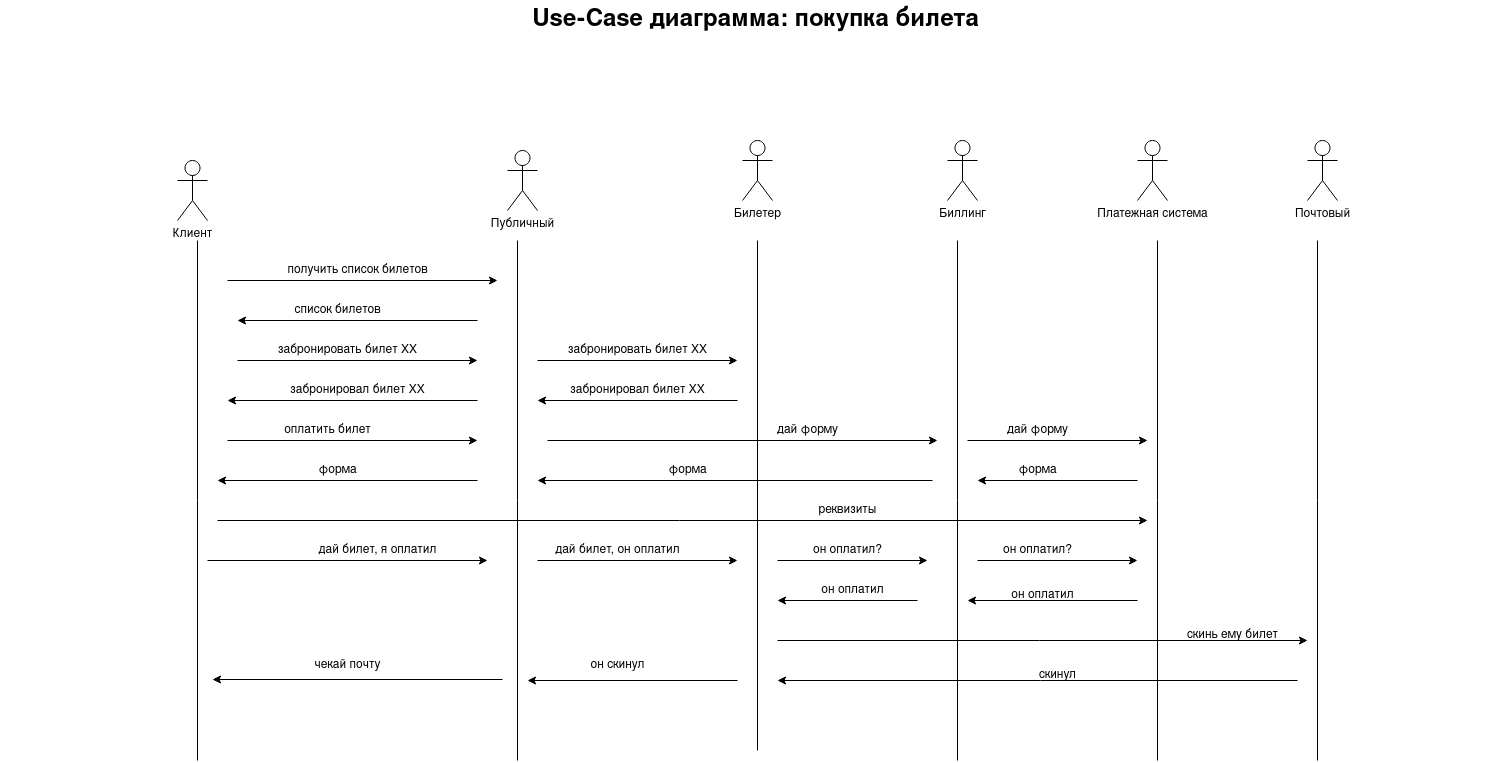
\includegraphics[width=16cm]{4-actions/use-case-payment.drawio.png}
      \centering
      \caption{Use-Case диаграмма: оплата билета}
\end{figure}

\begin{figure}
      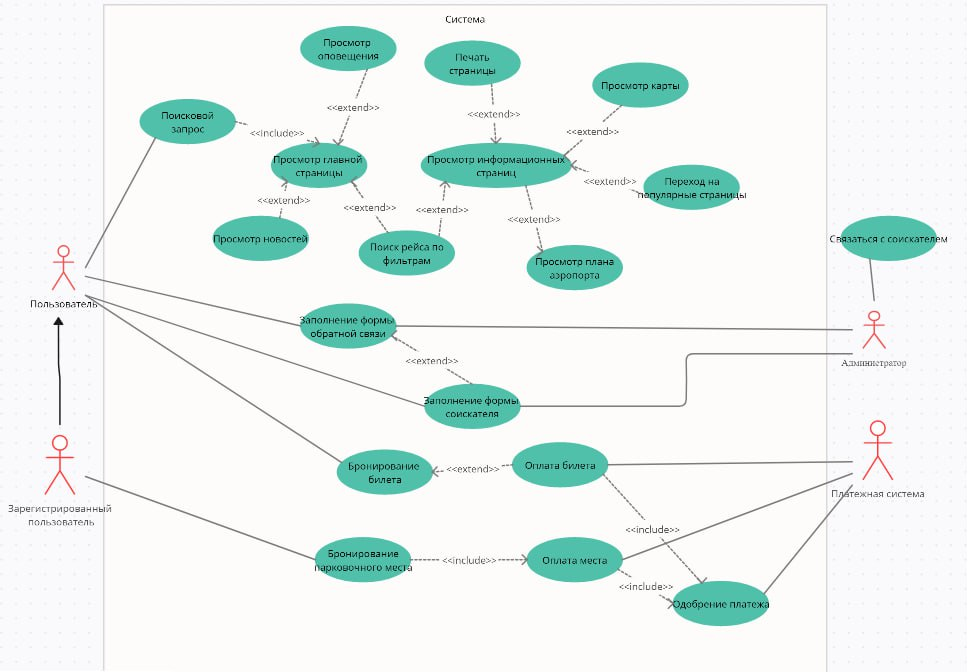
\includegraphics[width=16cm]{4-actions/use-case.jpg}
      \centering
      \caption{Use-Case диаграмма: вся система}
\end{figure}
